% !TEX TS-program = xelatex
%%%%%%%%%%%%%%%%%%%%% chapter.tex %%%%%%%%%%%%%%%%%%%%%%%%%%%%%%%%%
%
% sample chapter
%
% Use this file as a template for your own input.
%
%%%%%%%%%%%%%%%%%%%%%%%% Springer-Verlag %%%%%%%%%%%%%%%%%%%%%%%%%%
%\motto{Use the template \emph{chapter.tex} to style the various elements of your chapter content.}
%\chapter{Introduction to Solid Modeling}
%\label{intro} % Always give a unique label
%% use \chaptermark{}
%% to alter or adjust the chapter heading in the running head
%
%\abstract*{Each chapter should be preceded by an abstract (no more than 200 words) that summarizes the content. The abstract will appear \textit{online} at \url{www.SpringerLink.com} and be available with unrestricted access. This allows unregistered users to read the abstract as a teaser for the complete chapter.
%Please use the 'starred' version of the new |abstract| command for typesetting the text of the online abstracts (cf. source file of this chapter template |abstract|) and include them with the source files of your manuscript. Use the plain |abstract| command if the abstract is also to appear in the printed version of the book.}
%

\chapter{Introduction to Solid Modelers}
\label{chapt:intro}

In the last fifty years, Solid Modeling was conceived by engineers as a rigorous and universal language for geometry-based engineering.   Mathematically, at its core,  all solid models are computer representations of elements of some algebraic systems that are constructed and maintained by algorithms corresponding to the operations in the respective algebras~\cite{PAOLUZZI2023103436}.

The field focuses on the mathematical and computational models of solid shapes, of their morphology and topology, of their properties and behaviors, and of their aggregations into complex structures, such as those found in new micro-materials, in mechanical assemblies, or in large architectural projects. Solid Modeling provides a plethora of results and tools that impacts other Research fields, such as Robotics, Manufacturing, Architecture, Surgery Planning, Animation, and Computer Graphics~\cite{Rossignac:22:personal}.



\section{The Beginning}
\label{sec:1}



\subsection{Production Automation Project}
\label{subsec:1}


\paragraph{ccccccc}




\subsection{British Circle}
\label{subsec:2:style}



\paragraph{ccccccc}



\subsection{Manifold Representations}
\label{subsec:2:style}



\paragraph{ccccccc}



\section{Research and Academia}
\label{sec:2}


\subsection{Non-Manifold Representations}
\label{subsec:2:style}


\paragraph{ccccccc}



\subsection{First Industrial Modelers }
\label{subsec:2:style}


\paragraph{ccccccc}




\subsection{Modeling at IBM Research}
\label{subsec:2:style}


\paragraph{ccccccc}



\subsection{The European Branch}
\label{subsec:2:style}


\paragraph{France Industry}


\paragraph{Italian Academia}



\section{Modern Panorama}
\label{sec:3}


\paragraph{ccccccc}



\subsection{Product Lifecycle Management (PLM)}
\label{subsec:2:style}


\paragraph{ccccccc}



\subsection{Hollywood and Game Industry}
\label{subsec:2:style}


\paragraph{ccccccc}



\subsection{Two Competitor Kernels}
\label{subsec:2:style}

3D ACIS Modeler (ACIS) 

Parasolid

C3D Toolkit

Solid Modeling Solutions


\subsection{OpenSource CAD}
\label{subsec:2:style}


\paragraph{OpenCascade}


\paragraph{OpenCAD}


\paragraph{Blender}


\subsection{Building Information Modeling (BIM)}
\label{subsec:2:style}


\paragraph{Autodesk Revit}


\paragraph{Graphisoft ArchiCAD}


\paragraph{Scketchup}


\paragraph{Industry Foundation Classes (IFC)}


\paragraph{OpenBIM}


\paragraph{Blender OpenBIM (BlenderBIM)}



\subsection{Programming Language for Solid Modeling (PLASM)}
\label{subsec:2:style}

Many notation systems, called programming languages, are developed for writing computer programs. We can imagine their abstract set covered, in a mathematical sense, by a few subsets called \emph{programming paradigms} that characterize their \emph{programming style}, i.e., how the computation is performed, how data are transformed or stored, and other aspects of the calculation, globally known as the state of the computation.

Some languages follow a single paradigm; other languages are said to be multiparadigm since their programs may be written adopting more than one programming style. Examples are Smalltalk (object-oriented), Haskell or ML (functional), Prolog (declarative), C++, Java, Python, and Julia (multiparadigm). Modern languages tend to adapt flexibly to the most extensive array of problems and follow the programmer’s attitudes better.

Julia was designed for scientific programming, which currently it leads for performance, simplicity, and expressiveness, and quickly extended to accommodate most other programming paradigms. From the beginning it solved the \emph{two-language problem}~\cite{BEKS14}, that refers to prototyping with one slow dynamic language and rewrite it with a fast static language, so unifying program prototyping and optimization.

Therefore, Julia was the perfect choice for this book, oriented to teach geometric programming for  applications like computer-aided design and building information modeling. For this purpose, we ported as a package in Julia the geometric functional language |PLASM|~\cite{Paoluzzi:1995:GPP:212332.212349,Paoluzzi2003a}, derived from Backus’ FL, which we developed for supporting design, model generation, and visualization of geometric shapes, which are the environment of most scientific computations.


\subsubsection*{FP and FL}

John W. Backus directed the IBM team that invented and implemented the FORTRAN (Formula Translation) language. FORTRAN was the first high-level scientific and technical computer language developed by IBM in 1954-1956 for scientific and engineering applications and subsequently came to dominate scientific computing, and is used up to now on supercomputers.

The 1977 ACM Turing Award, in honor and recognition of Turing’s contribution to the field of computing, was presented to John Backus at the ACM Annual Conference in Seattle. In introducing the recipient, Jean E. Sammet, Chairman of the Awards Committee, said that  
it was for Fortran and the BNF (Backus Normal Form) that he was receiving that year's Turing Award.
Therefore, everybody was expecting Backus would describe the  work done to implement FORTRAN at IBM in the 1950s.

Conversely, the Backus’ Turing Lecture was entitled ``Can Programming Be Liberated from the von Neumann Style? A Functional Style and Its Algebra of Programs’’~\cite{10.1145/359576.359579}. This lecture was enormously influential, and opened a decade and half of renewed research work about functional languages. 


\begin{figure}
\centering
   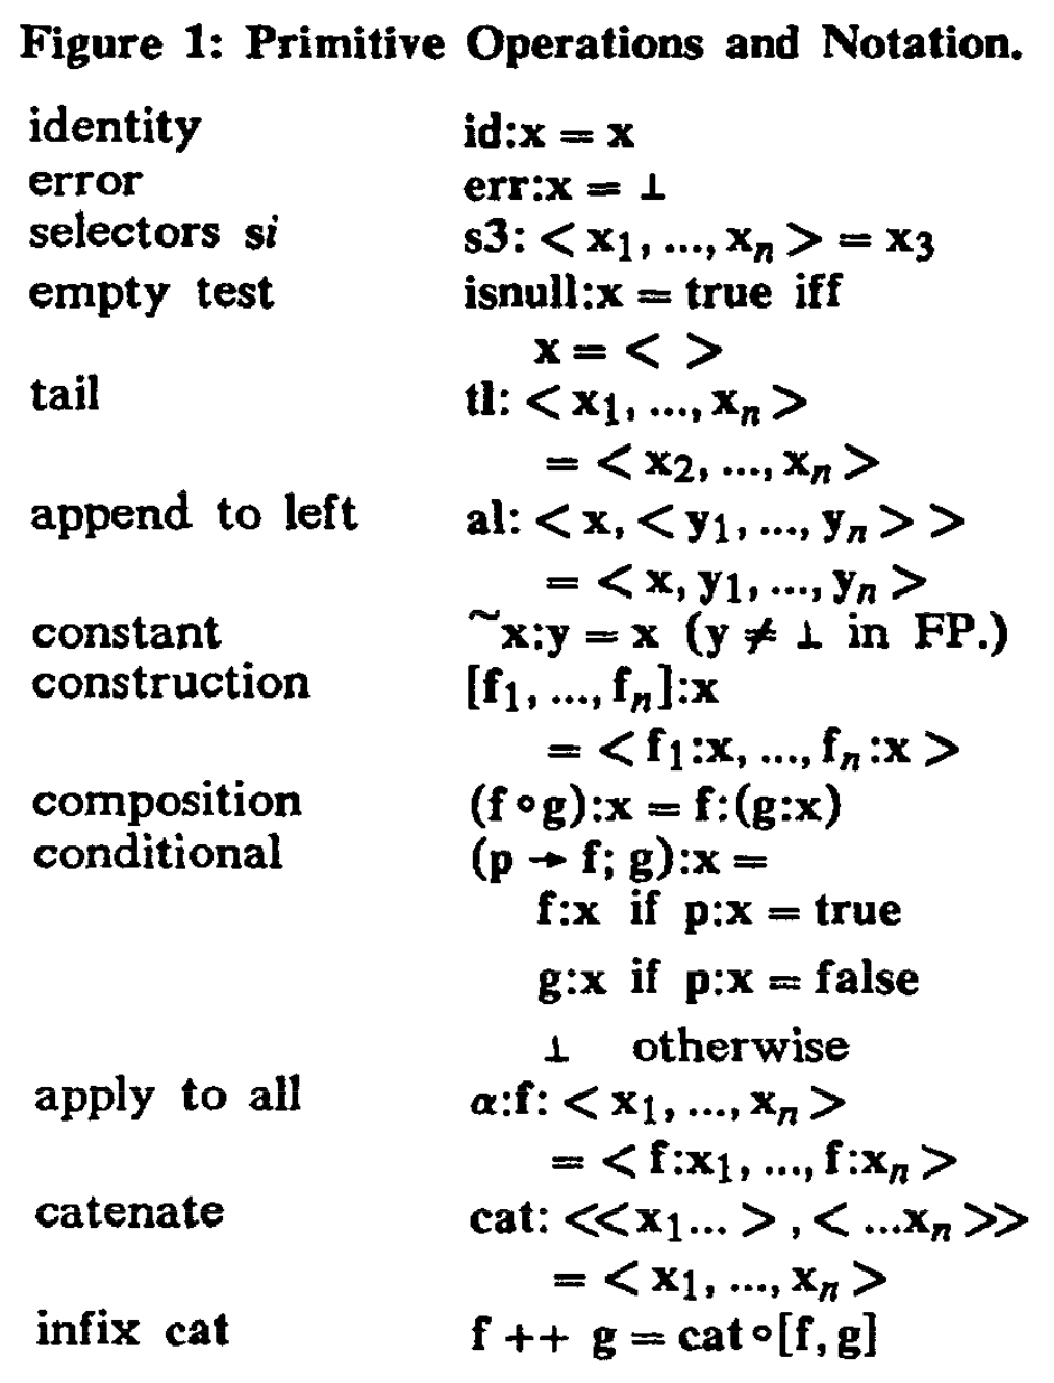
\includegraphics[width=2in]{chapter-01/figs/FP.pdf} \hfill~
\caption{The primitive operations (combining forms) and notations~\cite{10.1145/73560.73575} of FP programs. The semantics of FP is embodied in an underlying algebra of programs, a set of function level equalities that may be used to transform and to reason about programs.}
\label{fig:1:FP}
\end{figure}


A simple \emph{functional programming} (FP) system is described in~\cite{10.1145/359576.359579}. It is based on combining forms for building programs from simpler programs. An \emph{algebra of programs} is described whose variables denote FP functional programs and whose "operations" are FP functional forms, the combining forms of FP programs, to support the function-level programming paradigm. It allows building programs from a set of generally useful primitives and avoiding named variables. Only programs, aka functions, may be named. In Figure~\ref{fig:1:FP} we display the algebraic rules of FP.

FL (short for ``Function Level’’) is a programming language created by IBM Research at Almaden.
FL is the result of the effort~\cite{BWW90} to design a practical functional programming language based on Backus’ FP.  
FL is intended to be a programming language in which it is easy to write clear, concise,
and efficient programs. FL is designed around a rich set of functionals, forms for combining
existing programs to construct new ones. This emphasis on programming at the function
level results in programs that have a rich mathematical structure useful in reasoning about
and optimizing programs~\cite{IBM:RJ7100}.
A short description of FL combining forms  and primitive functions is given below, where its geometric extension with Julia’s functional syntax is discussed.

\subsubsection*{Classic PLaSM in Julia syntax}

Here we gives a brief informal description of the |PLASM| language, together with few examples. The section is intended to acquaint the reader with the syntax and style of |PLASM| programs without going into details. 

The interpreter and interactive GUI for PLASM were developed at the Sapienza University of Rome in the 1990s, extending the FL syntax and semantics with the only addition of a geometric type called Lar (hierarchical polyhedral complex) and supporting the FL programming style for geometric computing within the domain of Computer-Aided Design.

The book GP4CAD (Geometric programming for CAD)~\cite{Paoluzzi2003a} provides some hundreds of small, simple programs using the FL syntax.

In the past decade, the text-based user interface (TUI), the geometric computational kernel, and the interactive visualizer of ``classic’’ |PLASM| were ported to Python~\cite{pyplasm:2018} and C++, respectively, mainly using the functional features of such languages \cite{dia-report:2009}. Analogously, in recent times, a native and extended port to Julia is being carried out~\cite{plasm:2023}, used in this book, and briefly described in the following, abridged in a few general points.

\begin{enumerate}
\item Function \emph{application} and binary function \emph{composition} are native in Julia, which provides  |f($x$)| and  |g${}\circ{}$f|, respectively.
\item The FL \emph{sequence} |<$x_1, x_2, \ldots, x_n$>| is implemented as array |[$x_1, x_2, \ldots, x_n$]|.
\item All primitive functions (programs) are \emph{pure} (without side effects) and written \emph{uppercase}, while named expressions have capitalized names. 
\item Each |PLASM| function is \emph{unary}, possibly using an array of arguments. 
\item The geometric type |Lar| is extended with a Julia’s dictionary of properties.
\end{enumerate}


From~\cite{Paoluzzi2003a}, where the interested reader may find many codes discussed in this book in their FL version,  we recall that significant advantages are obtained with this approach in the style and efficiency of program developmen.
More generally, it is well known that functional programming enjoys several good properties:

\begin{itemize}
\item 
The set of syntax rules of a functional language is very small.
\item 
Each rule is very simple.
\item 
The program code is terse and clear.
\item 
The meaning of a program is well understood, since there is no state. 
\item 
Functions may be used both as programs and as data.
\item 
Programs are easily connected by concatenation and nesting.
\end{itemize}

\subparagraph{Programs are functions}\index{Programs are functions}

Generally speaking, a program is a \textit{function}.  When
\emph{applied} to some input \textit{argument}, a program
produces some output \textit{value}.  Two programs are usually
connected by using functional composition, so that the output of the
first program is used as input to the second program. Starting from here we use the Julia syntax.

\subparagraph{Program composition and application}\index{Program composition and application}

The composition of |PLASM| functions, i.e., |FL| programs with Julia syntax, works exactly as the composition of mathematical functions.  E.g., the application of the
composite mathematical function $f \circ g$ to the $x$ argument
\[
(f \circ g)(x) \equiv f(g(x))
\]
means that the function $g$ is first applied to $x$ and that the 
function $f$ is then applied to the value $g(x)$.  The |PLASM| notation 
for the previous expression is:
\begin{lstlisting}[language=JuliaLocal, style=julia, mathescape = true]
(f${}\circ{}$g)(x) $\equiv$ f(g(x))
\end{lstlisting}
where $\circ$ stands for binary function \textit{composition} and  
|g(x)| stands for \textit{application} of the function |g| to the 
argument |x|. Both notations are Julia’s native.


\subparagraph{Naming objects}\index{Naming objects}

In |PLASM|, a name can be assigned to every value generated by the
language, by using an (unmutable) \emph{definition} construct, either with or without
explicit parameters.  In both cases the so-called \textit{body} of the
definition, i.e.~the expression which follows the definition
\emph{head}, at the right hand of the ``|=|” symbol, will
describe the computational process which generates the  \emph{value}
produced by the computation.  The parameters which it
implicitly/explicitly depends on may be embedded in such a definition.
For example we may have
\begin{lstlisting}[language=JuliaLocal, style=julia, mathescape = true]
object = (Fun3 $\circ$ Fun2 $\circ$ Fun1)(params);
\end{lstlisting}
The computational process which produces the |object| value can be 
thought as the computational pipeline shown in 
Figure~\ref{fig:1:5:pipeline}.
\begin{figure}[htbp] %  figure placement: here, top, bottom, or page
   \centering
   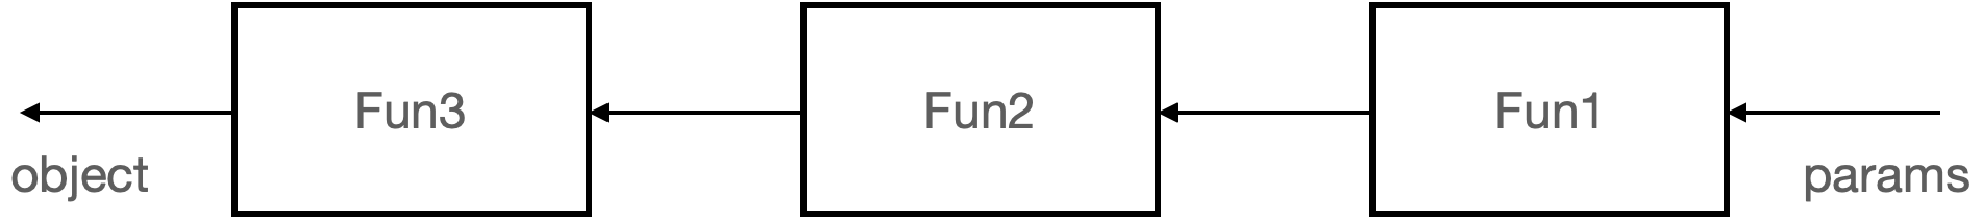
\includegraphics[width=0.8\textwidth]{chapter-01/figs/pipeline.pdf} 
	\caption{Example of computational pipeline}
   \label{fig:1:5:pipeline}
\end{figure}

In this example, the reliance of the model on the 
parameters is implicit.  To modify the generated object value 
it is necessary (a) to change the source code in either the body or 
the local environment of its generating function; (b) to compile the 
new definition; and (c) to evaluate again the object identifier.

\subparagraph{Parametrized objects}\index{Parametrized objects}

A \textit{parametric} geometric model can be defined, and easily
combined with other such models, by using a generating function with
{formal} \emph{parameters}.  Such kind of function may be instanciated
with different {actual} \emph{arguments}, thus obtaining different
output values.  For example, we may have:
\begin{lstlisting}[language=JuliaLocal, style=julia, mathescape = true]
object(params) = (Fun3 $\circ$ Fun2 $\circ$ Fun1)(params);

obj1 = object([p$_{1}$, p$_{2}$, $\ldots$ , p$_{n}$];
obj2 = object([q$_{1}$, q$_{2}$, $\ldots$ , q$_{n}$];
\end{lstlisting}
It is interesting to note that the generating function of a geometric
model may accept parameters of \emph{any} type, including other
geometric objects.



\subsubsection*{Geometric Programming at Function Level}
\label{sec:FL}

As we already know, |PLASM| is a geometry-oriented extension of a subset of
the |FL| language~\cite{BWW90,IBM:RJ7100}, which is a pure
functional language based on combinatory logic \href{https://en.wikipedia.org/wiki/Combinatory_logic}{[Wikipedia]}.  In particular, the
|FL| language makes use of both pre-defined and user-defined
\emph{combinators}, i.e. higher-order functions which are applied
to functions to produce new functions.  The small but very significant
|FL| subset which is used as the base environment of |PLASM| is summarized
in this section.  

Notice that here and in the remainder of this book the infix symbol
$\equiv$ is normally used to tell the reader that the
\emph{expression} on its left side evaluates to the \emph{value} on
its right side.  Sometimes this symbol is also used to denote an
equivalence between syntactical forms.




\subsubsection*{Elements of {FL} syntax in Julia}\index{Elements!of FL syntax}
\label{sec:FLsyntax}


Primitive |FL| \emph{objects} are characters, numbers and truth values.  Primitive objects added to it by |PLASM| are |Lar| geometric values.
Primitive objects, functions, applications and sequences are 
\emph{expressions}.
\emph{Sequences} are expressions separated by commas and contained within a pair
of square brackets (Julia |Vector| type):
\begin{lstlisting}[language=JuliaLocal, style=julia, mathescape = true]
[5, fun]
\end{lstlisting}

 An \emph{application} expression |exp1(exp2)| applies the 
\emph{function} resulting from the evaluation of |exp1| on the 
\emph{argument} resulting from the evaluation of |exp2|.  Julia 
allows some binary functions to be used both in infix and prefix form:
\begin{lstlisting}[language=JuliaLocal, style=julia, mathescape = true]
1 + 3 $\equiv$ +(1,3) $\equiv$ 4
\end{lstlisting}

 Application associates to left, i.e.~a sequence of repeated 
applications is evaluated from left to right. Note that this is only 
possible if all the applications, but possibly the last one, generate a 
new function to be applied to the next argument:
\begin{lstlisting}[language=JuliaLocal, style=julia, mathescape = true]
f(g)(h) $\equiv$ (f(g))(h)
\end{lstlisting}

 Application binds stronger than composition, i.e.~applications 
are evaluated first before compositions, as is shown in the 
following example.  Of course the application of |f| must generate a function value:
\begin{lstlisting}[language=JuliaLocal, style=julia, mathescape = true]
f(g) $\circ$ h $\equiv$ (f(g) $\circ$ h)
\end{lstlisting}


\subsubsection*{Combining forms and functions}\index{Combining forms and functions}
\label{subsec:2:forms}

The function level approach to programming of |FL| emphasizes the
definition of new functions by combining existing functions in various
ways.  The result of this approach is a programming style based on
function-valued expressions.  Some more important |FL| \emph{combining
forms} and functions follow.

\subparagraph{Construction}\index{Construction}

The combining form |CONS| allows application of a sequence
of functions to an argument, so producing a sequence of applications:  
\begin{lstlisting}[language=JuliaLocal, style=julia, mathescape = true]
CONS([f$_{1}$,...,f$_{n}$])(x) $\equiv$ [f$_{1}$(x),...,f$_{n}$(x)]
\end{lstlisting}
A |CONS|ed sequence of functions is a sort of \emph{vector function},
that can be composed with other functions and that can be applied to
data.  

E.g., |CONS([sin,cos,tan,atan])| when applied
to the argument |π| returns the sequence of applications
\begin{lstlisting}[language=JuliaLocal, style=julia, mathescape = true]
CONS([sin,cos,tan,atan])(π) 	#=
4-element Vector{Float64}:
  0.0
 -1.0
  0.0
  1.2626272556789115 	=#
\end{lstlisting}

\subparagraph{Apply-to-all}\index{Apply-to-all}
The combining form |AA| has a symmetric effect, i.e. it
applies a function to a sequence of arguments giving a sequence of applications. It is equivalent to the functional |map|  of other languages, Julia included:
\begin{lstlisting}[language=JuliaLocal, style=julia, mathescape = true] 
AA(f)([x$_{1}$,...,x$_{n}$]) $\equiv$ map(f, [x$_{1}$,...,x$_{n}$]) $\equiv$ [f(x$_{1}$),...,f(x$_{n})$]
\end{lstlisting}
For example, we may apply the trigonometric |SIN| function to all the elements of a 
list of numeric expressions:
\begin{lstlisting}[language=JuliaLocal, style=julia, mathescape = true] 
AA(SIN)([0, π/3, π/6, π/2]) 
$\equiv$ [SIN(0), SIN(π/3), SIN(π/6), SIN(π/2)]
$\equiv$ [0, 0.8660254037844382, 0.49999999999999956, 1.0];
\end{lstlisting}
The reader should notice that numeric computations often introduce
round-off and approximation errors.  Just remember that $\pi$ is an
irrational number and cannot be represented exactly by using finite
precision arithmetic.  Also, functions like |SIN| are computed
by using some truncated series expansion.

\subparagraph{Identity}\index{Identity}
The function  returns its argument unchanged
\begin{lstlisting}[language=JuliaLocal, style=julia, mathescape = true] 
ID(x) $\equiv$ x
\end{lstlisting}
In other words, the application of the identity function to \emph{any} argument, 
gives back the same argument:
\begin{lstlisting}[language=JuliaLocal, style=julia, mathescape = true] 
ID(0.5) $\equiv$ 0.5
ID(SIN) $\equiv$ SIN  
ID(SIN)(0) $\equiv$ SIN(0) $\equiv$ 0 
\end{lstlisting}


\subparagraph{Constant}\index{Constant}

The combining form |K| is evaluated as follows, for
whatever |x$_{1}$| and |x$_{2}$|: 
\begin{lstlisting}[language=JuliaLocal, style=julia, mathescape = true]
K(x$_{1}$)(x$_{2}$) $\equiv$ x$_{1}$
\end{lstlisting}
In other words, the first application returns a constant function of
value |x$_{1}$|, i.e.~such that when applied to \emph{any}
argument |x$_{2}$|, \emph{always} returns |x$_{1}$|. 
Some concrete examples follow:
\begin{lstlisting}[language=JuliaLocal, style=julia, mathescape = true] 
K(0.5) $\equiv$ Anonymous-Function 
K(0.5)(10) $\equiv$ 0.5 
K(0.5)(100) $\equiv$ 0.5 
K(0.5)(SIN) $\equiv$ 0.5 
\end{lstlisting}


\subparagraph{Composition}\index{Composition}

The binary composition of functions |COMP|, denoted in Julia by the symbol 
``$\circ$”, is defined in the standard mathematical way, as we already know:
\begin{lstlisting}[language=JuliaLocal, style=julia, mathescape = true]
(f $\circ$ g):x $\equiv$ f(g(x))
\end{lstlisting}
\emph{$n$-ary composition} of functions is also allowed:
\begin{lstlisting}[language=JuliaLocal, style=julia, mathescape = true]
COMP([f, g, h])(x) $\equiv$ (f $\circ$ g $\circ$ h)(x) $\equiv$ f(g(h(x)))
\end{lstlisting}
In the following we have, where |π|, |COS| and
|ACOS| are the |PLASM| denotations for $\pi$, |cos| and
|acos| \footnote{Which can be directly used in the \texttt{PLASM} code, of course.}, respectively:
\begin{lstlisting}[language=JuliaLocal, style=julia, mathescape = true]
(ACOS $\circ$ COS)(π) $\equiv$ ACOS(COS(π)) $\equiv$ ACOS(-1) $\equiv$ 3.141592653589793
(COS $\circ$ ACOS)(-1) $\equiv$ COS(ACOS(-1)) $\equiv$ COS(3.141592653589793) $\equiv$ -1
COMP([acos, cos, acos])(-1) $\equiv$ ACOS(COS(ACOS(-1))) $\equiv$ 3.141592653589793
\end{lstlisting}



\subparagraph{Conditional combinator}\index{Conditional}

This combinator has the
following semantic: ``|IF| the predicate |p| applied to object 
|x| is |true|, |THEN| apply |f| to
|x|; |ELSE| apply |g| to |x|". 
This construct is very useful when it is necessary to apply different
actions to input data depending on the value of some predicate
evaluated on them, and is possibly more ``natural" than the
conditional statements available in other languages.  

Formally, the conditional form |IF([ p, f, g ])| is evaluated as follows: 
\begin{lstlisting}[language=JuliaLocal, style=julia, mathescape = true]
IF([ p, f, g ])(x) 
	$\equiv$ f(x) if p(x) $\equiv$ TRUE
	$\equiv$ g(x) if p(x) $\equiv$ FALSE
\end{lstlisting}

From a syntax viewpoint, we remark that the |IF| operator is
a higher-order function that \emph{must} be applied to a
\emph{triplet of functions} in order to return a function which is in
turn applied to the input data.

A \emph{predicate} is a
function |p: T $\to \{true,
false\}\ \mbox{where}$ T $\mbox{is a}$ Type|.  Both
|true| and |false| are called \emph{truth values}, and
in Julia are |Bool| values. The predicate |p| is a \emph{function}, as well |f| and |g|,
to be alternatively executed depending on the truth value of the logical
expression |p(x)|.  E.g., we have:
\begin{lstlisting}[language=JuliaLocal, style=julia, mathescape = true]
    IF([ISINTPOS, K(true), K(false)])(1000) $\equiv$ true
    IF([ISINTPOS, K(true), K(false)])(-1000) $\equiv$ false
\end{lstlisting}
where |ISINTPOS| is a predefined predicate that returns |true| 
when applied to some positive integer. 


\subparagraph{Insert Right/Left}\index{Insert Right/Left}
The combining forms |INSR| and |INSL| allow the user to apply
a \emph{binary} function |f|, with signature\footnote{The \emph{signature}
of a function $f$ from a \emph{domain} $A$ to a \emph{codomain} $B$ is
the ordered pair of sets $(A,B)$.  It is normally associated to $f$ by
writing $f : A \rightarrow B$.} |f: D${}\times{}$D $\to$ D|, on a sequence
of arguments of \emph{any} length $n$. In other words, implicitly it is: |INSR(f): D$^n\to$ D|. Note that in the right-hand 
expressions below, |f| is always applied esplicitly  to a \emph{pair} of arguments:
\begin{lstlisting}[language=JuliaLocal, style=julia, mathescape = true] 
INSR(f)([x$_{1}$, x$_{2}$,$\ldots$, x$_{n}$]) $\equiv$ f([x$_{1}$, INSR(f)([x$_{2}$,$\ldots$, x$_{n}$])]) 
INSL(f)([x$_{1}$,$\ldots$, x$_{n-1}$, x$_{n}$]) $\equiv$ f([INSL(f)([x$_{1}$,$\ldots$, x$_{n-1}$]), x$_{n}$])
\end{lstlisting}

An interesting use example of the |INSL| combinator is given
below, where the function |BIGGER| : |Num| $\times$
|Num| $\to$ |Num| is defined.  The
|BIGGER| function returns the maximum of \emph{two} arguments; 
the |BIGGEST: Num|$^n \to$ |Num|  does the same from a list
of arguments of \emph{arbitrary length}:
\begin{lstlisting}[language=JuliaLocal, style=julia, mathescape = true] 
BIGGER   # predefined function
BIGGEST  = INSL(BIGGER)
SMALLER  # predefined function
SMALLEST = INSL(SMALLER)

BIGGER([-10, 0]) $\equiv$ 0 
BIGGEST([-10, 0, -100, 4, 22, -3, 88, 11]) $\equiv$ 88
\end{lstlisting}



\subparagraph{Catenate}\index{Catenate}
The |CAT| function appends to the first one any number of input sequences, so creating
a single output sequence:
\begin{lstlisting}[language=JuliaLocal, style=julia, mathescape = true]
CAT([[10,30,20],[11],[-7,8,12]]) $\equiv$ [10,30,20,11,-7,8,12])
\end{lstlisting}
A pair of concrete examples of how the |CAT| function is used
follows.  The second one is quite interesting: it gives a \emph{filter}
function used to select the non-negative elements of a number
sequence:
\begin{lstlisting}[language=JuliaLocal, style=julia, mathescape = true]
CAT([[10,30,20],[11],[-7,8,12]]) == [10,30,20,11,-7,8,12] 	#=
true	=#
(CAT ∘ AA(IF([ LT(0), K([]), ID ])))([-101,23,-37.02,0.1,84])
$\equiv$ CAT([ [], [23], [], [0.1], [84] ]) 
$\equiv$ [23, 0.1, 84]
\end{lstlisting}
It is useful to \emph{abstract} a |filter| function
with respect to a |predicate| and to an 
argument |sequence|, by showing this function semantics
where curried |LE| stands for \emph{less or equal} to its first argument. |LT|, |GE|, |GT| are similar.

\begin{lstlisting}[language=JuliaLocal, style=julia, mathescape = true]
FILTER(predicate)(sequence)
FILTER(LE(0))([-1,0,1,2,3,4]) == [-1, 0] # => true
\end{lstlisting}

\subparagraph{Distribute Right/Left}\index{Distribute Right/Left}
The functions |DISTR| and |DISTL|  are
defined as:  
\begin{lstlisting}[language=JuliaLocal, style=julia, mathescape = true]
DISTR([[a,b,c], x]) $\equiv$ [[a,x], [b,x], [c,x]]
DISTL([x, [a,b,c]]) $\equiv$ [[x,a], [x,b], [x,c]]
\end{lstlisting}
They accordingly transform a \emph{pair}, constituted by an arbitrary
expression  and by an arbitrary sequence, into a \emph{sequence
of pairs}.
\end{lstlisting}


\begin{script}
Let us give an example of |PLASM| use. The Euler number $e$ is defined as the 
sum of a series of numbers. In particular:
\[
e = {1\over 0!} + {1\over 1!} + {1\over 2!} + \cdots + {1\over n!} + \cdots
\]
We compute an \emph{approximation} of $e$, named |euler|,
as the sum of the first $21$ terms of the series.  The |factorial| function is native in 
Julia:
\begin{lstlisting}[language=JuliaLocal, style=julia, mathescape = true]
    euler = (ADD ∘ AA(DIV) ∘ DISTL)([1, AA(factorial)(0:20)])
\end{lstlisting}
The number 20 is the highest positive integer for which the expression |factorial(20)| does not overflow out of memory assigned to an |Int64| number. In Julia, you can use a type |BigInt| with the |big| function, converting a number to a maximum precision representation. 
Hence, redefine |factorial| as the |FACT| function below, which uses the \emph{ternary conditional} statement:

\begin{lstlisting}[language=JuliaLocal, style=julia, mathescape = true]
FACT(n) = n>0 ? *(1:big(n)...) : 1	#=
Fact (generic function with 1 method)	=#
FACT(100) #=
933262154439441526816992388562667004907159682643816214685929638
952175999932299156089414639761565182862536979208272237582511852
10916864000000000000000000000000	=#
\end{lstlisting}

The |euler| value is computed here by successive substitutions. Of course, the
Julia’s optimizing compiler might do a much better job:
\begin{lstlisting}[language=JuliaLocal, style=julia, mathescape = true]
euler = (ADD ∘ AA(DIV) ∘ DISTL)([1,AA(FACT)(0:9)])
$\equiv$ (ADD ∘ AA(DIV) ∘ DISTL)([1, AA(FACT)([0, 1, 2,$\ldots$, 8, 9])])
$\equiv$ (ADD ∘ AA(DIV) ∘ DISTL)([1, [FACT(0),FACT(1),$\ldots$,FACT(9)])])
$\equiv$ (ADD ∘ AA(DIV) ∘ DISTL)([1, [1,1,2,6,$\ldots$,40320,362880]])
$\equiv$ (ADD ∘ AA(DIV)(DISTL([1, [1,1,2,6,$\ldots$,40320,362880]]))
$\equiv$ (ADD ∘ AA(DIV)([[1,1], [1,1], [1,2], [1,6],$\ldots$,[1,362880]])
$\equiv$ ADD([ 1/1, 1/1, 1/2, 1/6, $\ldots$, 1/40320, 1/362880 ])
$\equiv$ 2.7182815255731922
\end{lstlisting}

Above, we have seen our first substantial example of |PLASM|, aka |FL| computation, as a sequence of expression transformations using the defining rules of combinators. The round brackets induce the order of transformations included into an expression and often corresponds to applications. The sub-expressions nested
more deeply are transformed first. When using |Float64|, i.e., 8 bytes, the numeric precision is 15-16 digits.

\vspace{5mm}
A simpler and more elegant implementation of the Euler number is given below, 
where |C| is the currying combinator\footnote{
In mathematics and computer science, \emph{currying} is the technique of translating the evaluation of a function that takes multiple arguments into evaluating a sequence of functions, each with a single argument.}:
\begin{lstlisting}[language=JuliaLocal, style=julia, mathescape = true]
    EULER(n) = (ADD ∘ AA(C(DIV)(1) ∘ FACT))(0:n)
\end{lstlisting}

The best Julia approximation of the Euler number is with |n = 57| terms of the defining series, since all  digits (80) of a |BigFloat| value are exact:

\begin{lstlisting}[language=JuliaLocal, style=julia, mathescape = true]
EULER(56)	#=
2.7182818284590452353602874713526624977549695416224291547344835
65013216246202514	=#
EULER(57)	#=
2.7182818284590452353602874713526624977549695416224291547344835
65013216246202549	=#
EULER(58)	#= The 58th element of the Euler series
2.7182818284590452353602874713526624977549695416224291547344835
65013216246202549	=#
\end{lstlisting}
\end{script}




\subsubsection*{Julia’s package Plasm.jl}

After many years of experimentation, a new Julia package is being developed while writing this book. We aim to finish the software version 1.0 before the book is published. The work has mainly consisted of porting to Julia the  Pyplasm library~\cite{} written in Python twelve years ago. Of course, both are open-source and downloadable from the web\footnote{Citation of pyplasm and plasm.jl URLs.}. Our software plan is to realize in version 1.0 a significant extension of the language related to computation of space arrangements~\cite{} and Boolean solid algebras~\cite{}.

Of course, the reader is warmly invited to install the latest version of Julia and to download our package |Plasm.jl| on the home machine. The installation is not strictly necessary since web access will be available. Still, it is always helpful, while learning a new language, to have your own environment where you are free to do any experiments.

\subparagraph{Plasm.jl}
The main file of the package is named as usual with the same name |Plasm.jl| of the package itself. Its primary function is to create the run-time executable of |Plasm.jl|, by calling the external references (i.e., the exported functionality) taken by other packages and to include the Julia code of other package files, in our case |fenvs.jl|, |hpc.jl|, and |viever.jl|. Note that its name starts uppercase, according to the Julia’s convention for packages.

\subparagraph{fenvs.jl}
The |fenvs.jl| file, whose name stands for “|f|unctional |env|ironment|s|” implements in Julia the majority of the small exciting programs developed for the GP4CAD book and includes many primitives for surface design with various methods. Other needed functions and functions of general use can be created directly by the reader if savant in computer graphics or CAD.

\subparagraph{hpc.jl}
The primary data structure is the |Lar| (Hierarchical Polyhedral Complex)~\cite{}, based on convex cells, and extended to allocate general polyhedral cells, i.e., polyhedra of any (low) dimension, connected but generally nonconvex and with interior holes. 
The |hpc.jl| file contains the developed design and implementation of the very general and \emp{multidimensional}  geometric data structure called |Lar|~\cite{}, that allows to accommodate all the geometric and solid algorithms and tools developed in this book. As we show in the book, the |Lar| structure is straightforward, versatile, and general. It does not use any of the large number of highly specialized and very complex data structures invented for solid modeling. We will show that our topological approach to geometric computations only needs the linear algebra of sparse matrices and vectors.

\subparagraph{viever.jl}
Finally, the |viewer.jl| file is used as the home of an interactive geometry viewer, used to interact with the shapes generated by Plasm codes either on the terminal screen of a laptop or on the HTML interface of a web browser program. This web viewer version was developed to view the Plasm models on the web and to write rich text examples and exercises within the web page of a web notebook, and hence without the need to install any software.





\subsubsection*{Geometric Programming examples}

\begin{coding}[2D virtual Manhattan] 
\label{example:1:Manhattan2D}

\begin{figure}
\centering
   
\includegraphics[width=0.59\textwidth]{chapter-01/figs/manhattan2d.pdf}%
   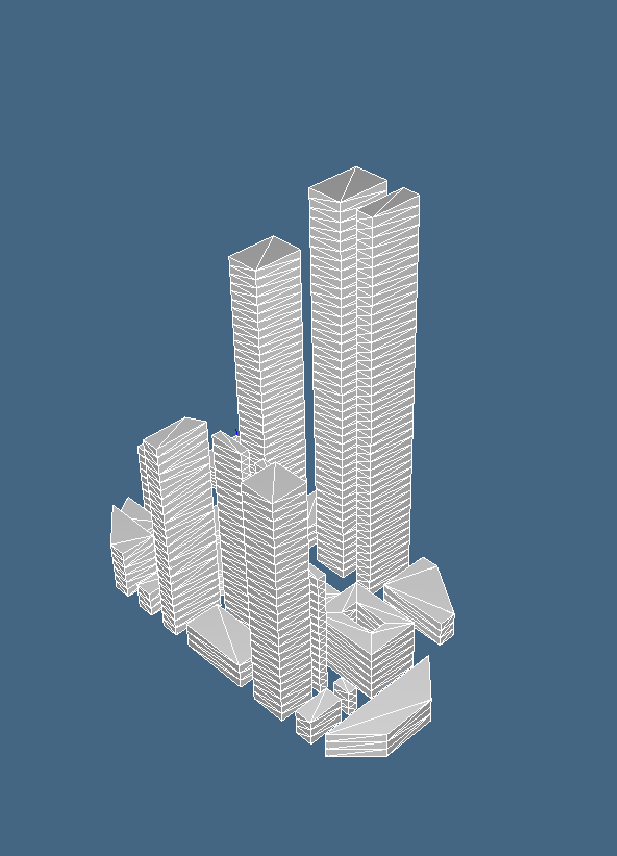
\includegraphics[width=0.41\textwidth]{chapter-01/figs/manhattan3d-1.pdf}

\caption{(a) Hierarchical polyhedral complex (Lar) 2D value embedded in 3D. A perspective projection generates the image. Each connected shape is a polyhedral cell, even nonconvex and with inner holes. Each triangle is a convex cell; (b) 3D model of Hpc type discussed in Example~\ref{example:1:Manhattan3D}}
\label{fig:1:FP}
\end{figure}

Of course, we started our geometric modeling session by telling the Julia compiler\footnote{To load \texttt{Plasm} in Julia, open a terminal, start your \texttt{julia} application, and after the prompt \texttt{julia>} write \texttt{using Pkg; Pkg.add("Plasm ")}} to use the |Plasm| package. Then, we give the compiler the code and data that follows, possibly contained in a file |Manhattan2D.jl|.

\begin{lstlisting}[language=JuliaLocal, style=julia, mathescape = true] 
julia> using Plasm
\end{lstlisting} 

We start by defining the 2D coordinates of the vertices of our model. 
\begin{lstlisting}[language=JuliaLocal, style=julia, mathescape = true] 
julia> verts = [[0.,0],[3,0],[5,0],[7,0],[8,0],[9.5,1],[10,1.5],[0,3],
[3,3],[5,3],[7,3],[8,3],[9.5,3],[0,4],[3,4],[5,4],[9.5,4],[12,
4],[9.5,5],[10,5],[12,5],[0,6],[3,6],[5,6],[0,7],[3,7],[5,7],
[9.5,7],[12,7],[9.5,8],[12,8],[0,9],[3,9],[5,9],[8,9],[9,9],[12,
9],[0,10],[3,10],[5,10],[8,10],[9,10],[9.5,10],[10,10],[12,10],
[6,11],[7,11],[0,12],[3,12],[9,12],[9.5,12],[0,13],[3,13],[6,
13],[7,13],[9,13],[9.5,13],[0,14],[3,14],[5,14],[8,14],[9,14],
[9.5,14],[10,14],[12,14],[0,15],[3,15],[5,15],[8,15],[0,16],[6,
16],[7,16],[9,17],[9.5,17],[10,17],[12,17],[6,18],[7,18],[9,18],
[9.5,18],[10,18],[12,18],[2,19],[3,19],[5,19],[8,19],[9,19],
[9.5,19],[10,19],[12,19],[5,20],[12,20],[7,22],[10,22],[9,6],
[12,6],[9,15],[9.5,15],[10,15],[12,15]]
\end{lstlisting}
Then we give the following description of convex cells on type |Cells = Vector{Vector{Int64}}|:
\begin{lstlisting}[language=JuliaLocal, style=julia, mathescape = true] 
julia> cells = [[1,2,9,8],[3,4,11,10],[5,6,13,12],[14,15,23,22],[16,
17,19,24],[7,18,21,20],[25,26,33,32],[27,95,28,35,34],[95,96,29,
28],[30,31,37,36],[38,39,49,48],[40,41,47,46],[41,61,55,47],[55,
61,60,54],[54,60,40,46],[42,43,51,50],[44,45,65,64],[52,53,59,
58],[56,57,63,62],[66,67,84,83,70],[68,69,72,71],[69,86,78,72],
[78,86,85,77],[71,77,85,68],[97,98,74,73],[99,100,76,75],[79,80,
88,87],[81,82,90,89],[91,92,94,93]]
\end{lstlisting}
Finally, |verts|  and |cells| are transformed in a geometric object of type |Hpc| 
by the function |MKPOL| and stored in the Julia variable named |model|.

\begin{lstlisting}[language=JuliaLocal, style=julia, mathescape = true] 
julia> model = MKPOL(verts,cells)
# Hpc
\end{lstlisting}
A |model| image is then generated in the interactive |Plasm| viewer, within a system window named "Manhattan2D”, for interaction with mouse and arrow buttons. From terminal we might do: \$| julia path/Manhattan2D.jl|
\begin{lstlisting}[language=JuliaLocal, style=julia, mathescape = true] 
julia> VIEW( model, "Manhattan2D” )
\end{lstlisting}

\end{coding}



\begin{figure}
   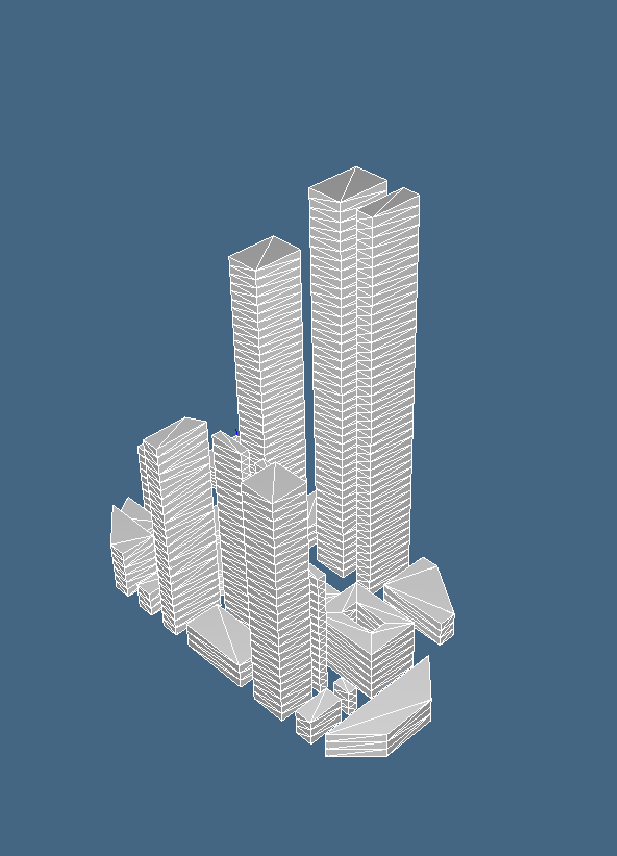
\includegraphics[width=1.955in]{chapter-01/figs/manhattan3d-1.pdf}
   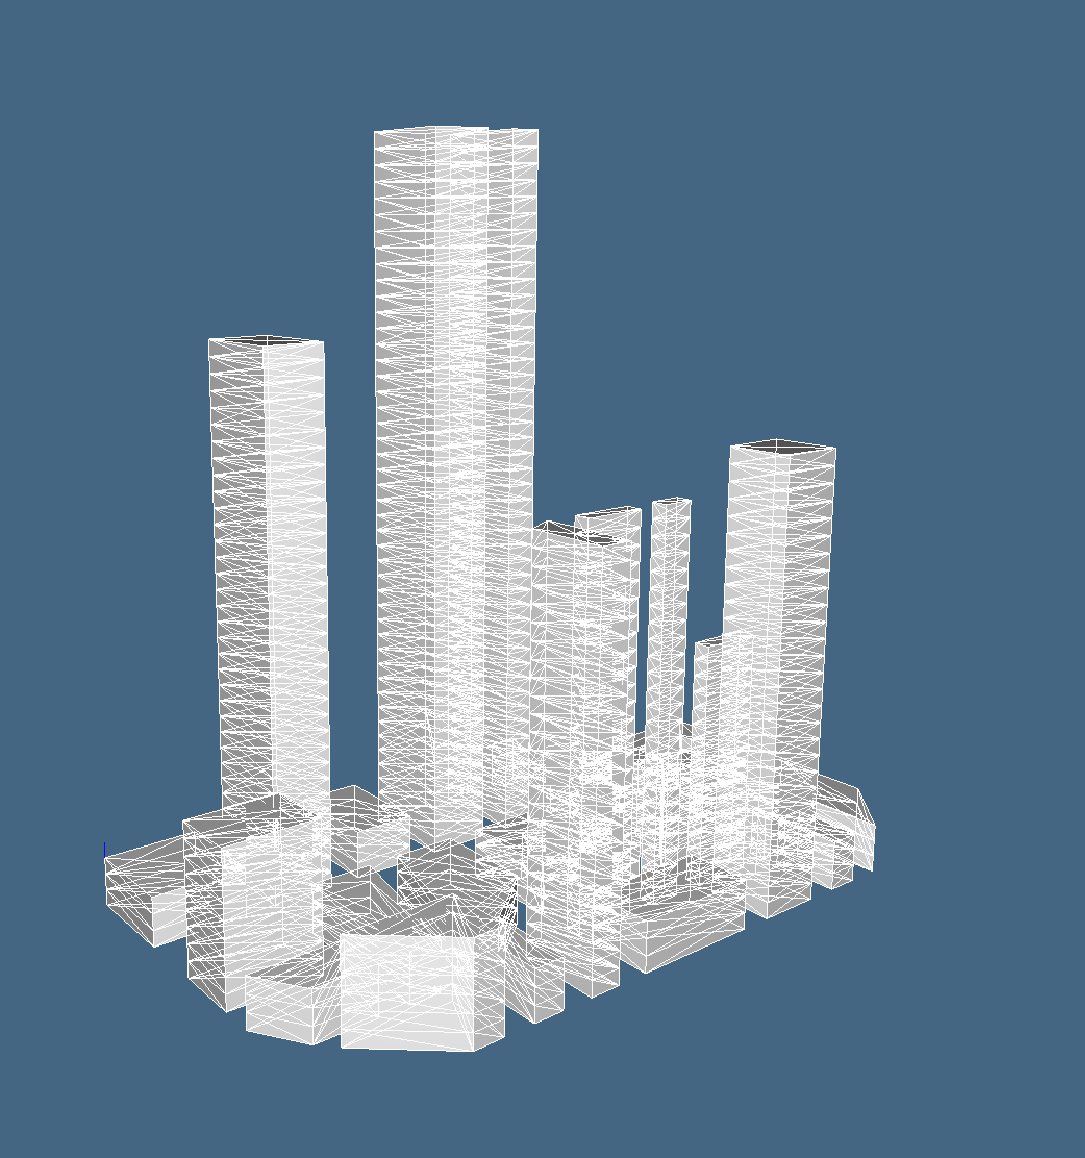
\includegraphics[width=2.55in]{chapter-01/figs/manhattan3d-2.pdf}
\caption{3D model generated by using the 2D \texttt{cells} defined in \texttt{Manhattan2D} example.
 (a) opaque visualization; (b) transparent visualization from a different viewpoint.}
\label{fig:1:FP3D}
\end{figure}

\begin{coding}[3D virtual Manhattan] 
\label{example:1:Manhattan3D}

The model of Figure~\ref{fig:1:FP3D} is given by (1) a vector |ManhattanH| of numbers; (2) generation of 1D and 2D arrays of |Hpc| objects stored in |pols1D| and |pols2D|, respectively; (3)~by Cartesian product of all the |Hpc| pairs |(2D,1D)|. See the code below:

\begin{lstlisting}[language=JuliaLocal, style=julia, mathescape = true] 
ManhattanH = [1,3,1,11,1,2,1,1,1,8,15,1,1,1,1,8,1,15,8, 1,2,2,2,2,5,9,1,1,1].*3
# 29-element Vector{Int64}:
storeys = CONS(AA(DIESIS)(ManhattanH))(.5)
# 29-element Vector{Vector{Float64}}:
pols1D = AA(QUOTE)(storeys)
# 29-element Vector{Hpc}:
pols2D = [MKPOL(verts,[cell]) for cell in cells]
# 29-element Vector{Hpc}:
pols3D = AA(splat(*))(TRANS([pols2D, pols1D]))
# 29-element Vector{Hpc}:
VIEW(STRUCT(pols3D), "Manhattan3D")
\end{lstlisting}


In particular, we define an array of virtual heights for each \emph{polygon} of |Manhattan2D|. Such numbers are transformed in repeated | stories | heights by |AA(DIESIS)| (|DIESIS| was the |#| operator in |FL|-based |PLASM|, not usable in Julia, since it denotes comments) and then codified as 1D |Hpc| polyhedra stored in |pols1D| by the |QUOTE| operator. Analogously, a set of 2D polyhedra is stored in the |pols2D| array. The Cartesian product |(*)| of every pair of corresponding |Hpc| objects is stored in |pols3D| array using the Julia’s |splat| function. Finally, a single |Hpc| object is visualized in a system window named |Manhattan3D|. 

It is worth noting that every |polygon*segment| multiplication of two |Hpc| objects produces a new |Hpc| polyhedron of dimension equal to the sum of dimensions of operands.
The reader should not forget that the |PLASM| language and the |Hpc| data structure are both  \emph{multidimensional}.

We also note that a large number of significant programming examples with Julia and |PLASM| in Julia can be found inside the file |fenvs.jl|, and executed in the terminal by writing \$ |julia ./test/fenvs.jl|, being located into the |Plasm.jl directory|, and after having downloaded and installed the package |Plasm.jl| in a recent |julia| environment.
\end{coding}

\begin{coding}[A canonical curved example]

\begin{figure}[htbp]
\centering
   
\includegraphics[width=\textwidth]{chapter-01/figs/functionmap.pdf} \hfill~
\caption{The mapping of a function of two arguments on its 2D parameter domain. Each element (point and cell) of the cellular domain is paired with a corresponding element in the function range. The figure shows how the elements are paired. (a) The cellular complex decomposing the function domain $[2\pi,1]$; (b) the function range transformed after the function \texttt{p->[u,sin(u)∗v]} was mapped on the vertices of the 2D domain. }
\label{fig:1:sinmapping}
\end{figure}

A very simple geometric example is given here, showing some of canonical constructs of geometric design with |Plasm|. First, we build and show in Figure~\ref{}a the  |Domain2D| of the parametric 2D solid |model| given in Figure~\ref{}b.  The |MAP| operator needs to be applied first to the function |Mapping2D| to be applied to all \emph{vertices} of a cell decomposition of |Domain2D|, in turn generated as the Cartesian product (|POWER|) of two 1D cellular complexes, so producing a 2D cell decomposition. 

\begin{lstlisting}[language=JuliaLocal, style=julia, mathescape = true] 
Domain2D = Power(INTERVALS(2π)(36), INTERVALS(1)(6));
Mapping2D = p->((u,v)=p; [u,sin(u)*v]);
model = MAP(Mapping2D)(Domain2D)
\end{lstlisting}

The two parameters |u,v| of the model domain are worked out by |p->(...)|, anonymous |Julia| function, and applied to each vertex of |Domain2D| by the |MAP| operator.
The virtual models of both |Domain2D| and |model|, finally visualized in Figure~\ref{}, are made available for display by the |Plasm| operator |VIEW|, and can be interactively handled by the user.

\begin{lstlisting}[language=JuliaLocal, style=julia, mathescape = true] 
VIEW(Domain2D)
VIEW(model)
\end{lstlisting}
\end{coding}



\bibliographystyle{spmpsci}
\bibliography{book.bib}


%
%\end{document}
%
